\tikzstyle{mybox} = [draw=black, fill=white, very thick,
    rectangle, rounded corners, inner sep=10pt, inner ysep=10pt]
\tikzstyle{fancytitle} =[fill=black, text=white, font=\bfseries]
%\newcommand*\bigcdot{\mathpalette\bigcdot@{.5}}
%\newcommand*\bigcdot@[2]{\mathbin{\vcenter{\hbox{\scalebox{#2}{$\m@th#1\bullet$}}}}}

\begin{multicols*}{2}


%------------ Length ---------------
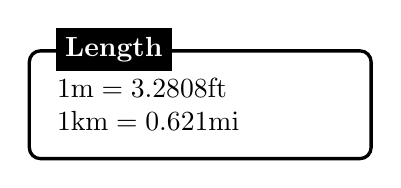
\begin{tikzpicture}
\node [mybox] (box){%
    \begin{minipage}{0.3\textwidth}
    ${\rm 1 m = 3.2808 ft }$ \\
    ${\rm 1 km = 0.621 mi }$ 
    \end{minipage}
};
\node[fancytitle, right=10pt] at (box.north west) {Length};
\end{tikzpicture}

%------------ Volume ---------------
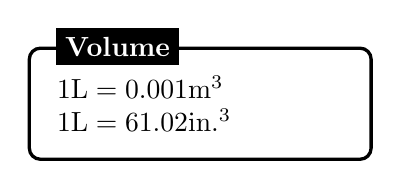
\begin{tikzpicture}
\node [mybox] (box){%
    \begin{minipage}{0.3\textwidth}
    ${\rm 1 L = 0.001 m^3 }$\\
    ${\rm 1 L = 61.02 in.^3}$
    \end{minipage}
};
\node[fancytitle, right=10pt] at (box.north west) {Volume};
\end{tikzpicture}

%------------ MASS ---------------
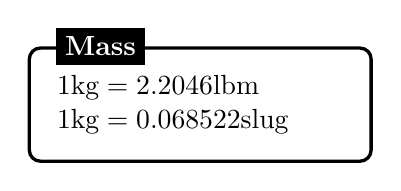
\begin{tikzpicture}
\node [mybox] (box){%
    \begin{minipage}{0.3\textwidth}
    ${\rm 1 kg = 2.2046 lbm }$\\
    ${\rm 1 kg  = 0.068 522 slug }$
    \end{minipage}
};
\node[fancytitle, right=10pt] at (box.north west) {Mass};
\end{tikzpicture}


%------------ Force ---------------
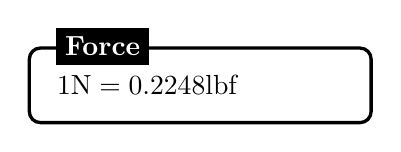
\begin{tikzpicture}
\node [mybox] (box){%
    \begin{minipage}{0.3\textwidth}
    ${\rm 1 N = 0.2248 lbf }$
    \end{minipage}
};
\node[fancytitle, right=10pt] at (box.north west) {Force};
\end{tikzpicture}


%------------ Work/Energy ---------------
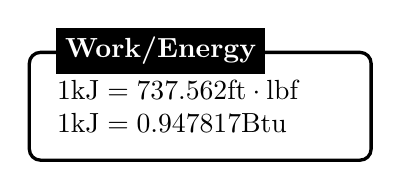
\begin{tikzpicture}
\node [mybox] (box){%
    \begin{minipage}{0.3\textwidth}
    ${\rm 1 kJ = 737.562 ft \cdot lbf  }$ \\
    ${\rm 1 kJ = 0.947 817 Btu }$
    \end{minipage}
};
\node[fancytitle, right=10pt] at (box.north west) {Work/Energy};
\end{tikzpicture}


%------------ Pressure/Stress ---------------
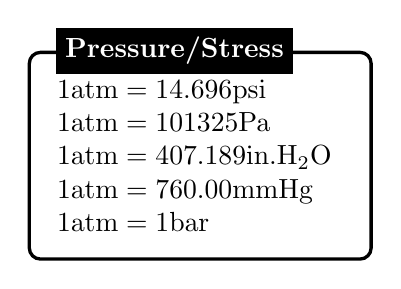
\begin{tikzpicture}
\node [mybox] (box){%
    \begin{minipage}{0.3\textwidth}
    ${\rm 1 atm = 14.696 psi }$ \\
    ${\rm 1 atm = 101 325 Pa }$ \\
    ${\rm 1 atm = 407.189 in. H_2O }$ \\ 
    ${\rm 1 atm = 760.00 mm Hg }$ \\ 
    ${\rm 1 atm = 1 bar }$
    \end{minipage}
};
\node[fancytitle, right=10pt] at (box.north west) {Pressure/Stress};
\end{tikzpicture}


%------------ Density ---------------
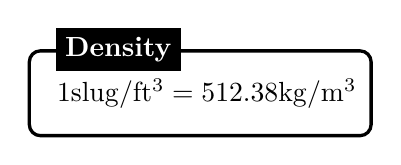
\begin{tikzpicture}
\node [mybox] (box){%
    \begin{minipage}{0.3\textwidth}
    ${\rm 1 slug/ft^3 = 512.38 kg/m^3  }$ 
    \end{minipage}
};
\node[fancytitle, right=10pt] at (box.north west) {Density};
\end{tikzpicture}

%------------ Temperature ---------------
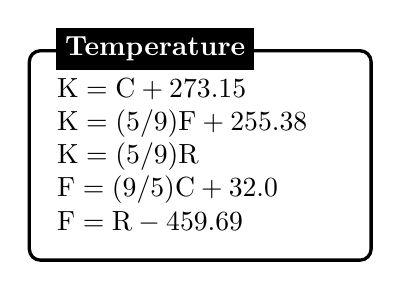
\begin{tikzpicture}
\node [mybox] (box){%
    \begin{minipage}{0.3\textwidth}
    ${\rm K = ° C +273.15  }$ \\
    ${\rm K = (5/9) × ° F + 255.38  }$ \\
    ${\rm K = (5/9) × ° R  }$ \\
    ${\rm ° F = (9/5) × ° C + 32.0  }$ \\
	${\rm ° F = ° R - 459.69 }$
    \end{minipage}
};
\node[fancytitle, right=10pt] at (box.north west) {Temperature};
\end{tikzpicture}

%------------ Scales ---------------
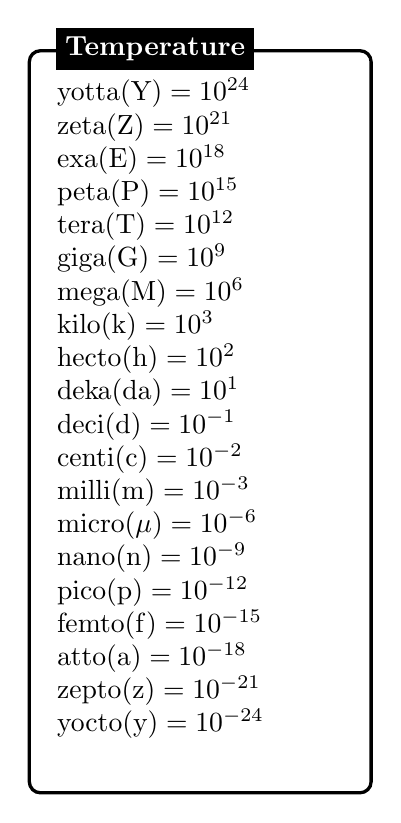
\begin{tikzpicture}
\node [mybox] (box){%
    \begin{minipage}{0.3\textwidth}
    ${\rm yotta (Y) = 10^{24}  }$ \\
    ${\rm zeta (Z) = 10^{21}  }$ \\
    ${\rm exa (E) = 10^{18}  }$ \\
    ${\rm peta (P) = 10^{15}  }$ \\
    ${\rm tera (T) = 10^{12}  }$ \\
    ${\rm giga (G) = 10^{9}  }$ \\
    ${\rm mega (M) = 10^{6}  }$ \\
    ${\rm kilo (k) = 10^{3}  }$ \\
    ${\rm hecto (h) = 10^{2}  }$ \\
    ${\rm deka (da) = 10^{1}  }$ \\
    ${\rm deci (d) = 10^{-1}  }$ \\
    ${\rm centi (c) = 10^{-2}  }$ \\
    ${\rm milli (m) = 10^{-3}  }$ \\
    ${\rm micro (\mu) = 10^{-6}  }$ \\
    ${\rm nano (n) = 10^{-9}  }$ \\
    ${\rm pico (p) = 10^{-12}  }$ \\
    ${\rm femto (f) = 10^{-15}  }$ \\
    ${\rm atto (a) = 10^{-18}  }$ \\
    ${\rm zepto (z) = 10^{-21}  }$ \\
    ${\rm yocto (y) = 10^{-24}  }$ \\
    \end{minipage}
};
\node[fancytitle, right=10pt] at (box.north west) {Temperature};
\end{tikzpicture}

\end{multicols*}
